% !Mode:: "TeX:UTF-8"
%!TEX program  = xelatex

\documentclass{cumcmthesis}
%\documentclass[withoutpreface,bwprint]{cumcmthesis} %去掉封面与编号页
\usepackage{subfig}
\usepackage{url}
\usepackage{amsmath}
\usepackage{graphicx}%图片
\title{多波束测线问题}
\tihao{B}
\baominghao{6666}
\schoolname{西安电子科技大学}
\membera{孟文堂}
\memberb{谢小凡}
\memberc{魏朝旭}
\supervisor{XXX老师}
\yearinput{2024}
\monthinput{08}
\dayinput{08}

\begin{document}

 \maketitle
 \begin{abstract}
 	
本文针对\textbf{生鲜商超}中蔬菜类商品的自动定价与补货决策问题，运用数据分析、时间序列分析、聚类分析以及优化算法等方法，建立了\textbf{蔬菜销售预测}模型、\textbf{成本加成定价}模型以及利润最大化模型。通过销售数据的统计分析，得到了单品和品类的销售分布规律及其相互关系；通过时间序列分析，识别了销售量的季节性周期；利用K-means++聚类算法，对单品进行了市场细分；最终，通过优化算法（如LINGO和遗传算法）求解出了未来一周的补货总量和定价策略，以及特定日期的单品补货量和定价，较好地解决了商超的\textbf{补货和定价优化}问题。

针对问题一，首先通过计算三年内各单品的总销售量，得到了单品销售分布规律，并取前二十位进行分析；其次，利用系统聚类谱系图和K-means++算法，对单品进行了聚类分析，识别出不同的销售群体；同时，绘制了品类销售量的折线图，揭示了其季节性周期规律；最后，通过\textbf{Spearman相关系数}，计算了各品类之间的相关性，揭示了它们之间的市场关联。

针对问题二，首先计算了每个品类每天的总销售量和加权平均价格，通过曲线拟合建立了销售量和价格的关系函数；然后，利用历史数据预测了未来一周的销售量，并通过关系函数预测了相应的平均价格；最后，构建了\textbf{利润最大化}模型，使用优化算法求解出了各品类的最优补货量和定价策略，实现了商超收益的最大化。

针对问题三，首先预测了7月1日各单品的销售量，然后结合最小陈列量要求和商超销售空间限制，构建了单品补货和定价的优化模型；通过\textbf{遗传算法}求解该模型，得到了满足市场需求且使商超收益最大的单品补货量和定价策略。

针对问题四，为了更好地制定蔬菜商品的补货和定价决策，商超还需要采集实时库存数据、供应商信息、顾客购买行为数据、竞争对手信息以及市场趋势数据等。这些数据有助于商超更准确地预测市场需求、优化库存管理、降低采购成本、提高顾客满意度以及增强市场竞争力。本文所运用的模型优点在于能够综合考虑多种因素，为商超提供科学的决策支持；但同时，模型的准确性和有效性也依赖于数据的完整性和准确性，以及算法的选择和参数设置。因此，在实际应用中，需要根据具体情况对模型进行调整和优化。

\keywords{蔬菜销售预测\quad Spearman相关系数\quad 利润最大化\quad 补货和定价优化\quad 遗传算法}
\end{abstract}

%目录
%\tableofcontents
%\newpage
\section{问题重述}

\subsection{问题背景}

在生鲜商超的复杂运营生态中，蔬菜类商品的管理构成了其日常运营的核心挑战之一。蔬菜作为生鲜商品中的关键组成部分，其保鲜期短、外观品质敏感，且市场需求波动剧烈，极易受到季节变换、天气状况、节假日效应以及消费者偏好等多重因素的共同影响。这种高度的市场敏感性与不确定性，使得蔬菜的库存控制与定价策略成为了一项极具挑战性的任务。

传统的生鲜商超管理往往依赖于经验判断与直觉决策，难以精准捕捉市场需求的微妙变化，从而容易导致库存积压与缺货现象并存的问题。库存积压不仅增加了商超的运营成本与损耗风险，还可能影响商品的新鲜度与品质，进而损害顾客的消费体验与满意度；而缺货则可能错失销售机会，降低顾客忠诚度与市场份额。

因此，如何运用现代数学方法与数据分析技术，构建一套科学、高效的蔬菜商品补货与定价决策支持系统，成为生鲜商超行业亟待解决的重要课题。

\subsection{问题内容}

本研究以生鲜商超的蔬菜类商品为研究对象，基于历史销售数据、市场趋势、成本结构以及顾客需求等信息，建立数学模型，以解决以下关键问题：

（1）\textbf{蔬菜销售分布与关联性分析}：通过统计分析方法，揭示各品类及单品蔬菜的销售分布规律，并探讨它们之间的销售关联，为后续的补货和定价决策提供数据支持。

（2）\textbf{品类补货量与定价策略制定}：基于成本加成定价原则和市场预测，建立模型以预测未来一周内各蔬菜品类的销售总量，并制定相应的日补货总量和定价策略，旨在实现商超收益的最大化。

（3）\textbf{单品补货量与定价优化}：在考虑到销售空间限制、最小陈列量要求以及市场需求预测的前提下，建立优化模型以确定特定日期（如7月1日）各单品的补货量和定价，以平衡供需关系并提升顾客满意度。

（4）\textbf{数据需求与决策优化探索}：分析现有数据的局限性，探讨商超为了改进补货与定价决策还需采集的额外数据类型（如实时库存数据、顾客购买行为数据等），并评估这些数据对优化决策模型的潜在贡献。

\section{问题分析}

\subsection{蔬菜销售分布与关联性分析}

在蔬菜销售分布与关联性分析阶段，我们计划首先通过计算三年来每个单品的总销售量，并进行排序，以揭示单品销售量的分布情况。这一步骤将帮助我们识别出畅销品和滞销品，为后续的库存管理提供依据。

对于单品之间的相互关系，我们打算采用系统聚类分析方法，特别是K-means++算法，对三年的销售额数据进行聚类分析。通过聚类，我们可以将单品划分为不同的群组，这些群组内的单品在销售上可能具有相似的特性或趋势。聚类结果将为我们提供关于单品之间相互关系的深入理解，有助于商超在促销和货架布局方面做出更合理的决策。

在品类层面，我们将以天为时间单位，分析每个品类每日的销售总量，并绘制折线图以展示其变化趋势。通过观察折线图，我们可以发现品类销售的季节性波动和其他潜在规律。为了量化品类之间的相互关系，我们计划采用Spearman相关系数，因为它不依赖于数据的正态性假设，适用于我们可能遇到的非正态分布数据。通过计算每两个品类之间的相关系数，我们可以得出它们之间的正相关、负相关或无相关关系，为商超的品类管理和促销策略提供科学依据。

\textbf{选择该思路的原因}：聚类分析和Spearman相关系数是分析销售数据的有效工具，它们能够揭示数据中的内在结构和关系，为决策提供有力支持。同时，这些方法具有较强的灵活性和适应性，能够处理不同类型和规模的数据集。

\subsection{品类补货量与定价策略制定}

为了制定科学合理的品类补货量与定价策略，我们计划首先利用历史销售数据建立销售量与平均价格之间的关系函数。这一函数将帮助我们预测未来销售量和平均价格的变化趋势。随后，我们将利用这些预测结果和利润函数，通过优化求解方法来制定最优的补货量与定价策略。

在优化求解过程中，我们考虑使用LINGO等优化软件，因为它们具有强大的求解能力和灵活的建模方式，能够处理复杂的优化问题。通过设定供给量小于等于销售量的约束条件，并最大化利润为目标函数，我们可以求得最优的补货量与定价策略。

\textbf{选择该思路的原因}：曲线拟合、预测分析和优化求解是制定补货量与定价策略的有效方法。它们能够综合考虑多个因素（如销售量、价格、成本等），并在约束条件下求出最优解。同时，利用优化软件可以大大提高求解效率和准确性。

\subsection{单品补货量与定价优化}

对于单品补货量与定价的优化问题，我们计划采用预测分析与启发式搜索算法（如遗传算法）相结合的方法。首先，我们将利用历史销售数据预测特定日期（如7月1日）各单品的销售量。然后，设定目标函数（如最大化收益）和约束条件（如库存限制、陈列量要求等），通过遗传算法等启发式搜索算法来求解最优的补货量与定价策略。

\textbf{选择该思路的原因}：遗传算法等启发式搜索算法具有全局搜索能力强、鲁棒性好的优点，能够在复杂的约束条件下有效地搜索最优解。同时，这些算法易于实现且参数调整灵活，非常适合处理此类具有多个变量和约束条件的优化问题。

\subsection{数据需求与决策优化探索}

在数据需求与决策优化方面，我们认识到商超需要不断拓展和整合数据来源以提高决策的准确性和科学性。除了现有的销售数据外，商超还应关注实时库存数据、顾客购买行为数据、供应商信息、市场趋势数据等多种数据源。这些数据将有助于商超更全面地了解市场需求和竞争态势，为制定更加精准的补货与定价策略提供有力支持。

为了充分利用这些数据资源并提升决策系统的智能化水平，我们建议商超建立全面的数据治理体系和数据分析团队，并积极探索新的数据分析技术和方法（如机器学习、深度学习等）。这将有助于商超在激烈的市场竞争中保持领先地位并实现可持续发展。

\section{模型的假设}

\begin{itemize}
\item 	\textbf{数据可靠性与代表性}：销售、库存、价格等数据完整、准确，能代表过去并预测未来趋势，且市场环境无重大不可预见变化。
\item 	\textbf{市场需求与价格弹性}：消费者购买行为稳定，价格与销售量间存在可预测的弹性关系，且在一定时间内保持稳定。
\item 	\textbf{库存与成本管理}：商超具备有效库存管理，能及时补货，库存成本可预测。
\item 	\textbf{销售策略有效性}：促销、折扣等策略能提升销售量，其成本与收益可量化。
\item 	\textbf{竞争环境稳定}：竞争对手行为稳定，商超具备市场竞争力，能抵御外部压力。
\item 	\textbf{成本与利润线性关系}：销售收入与成本之间的差额构成利润，且这一关系在模型中可明确描述。
\item 	\textbf{模型适用性与局限}：模型适用于当前销售环境，能预测趋势并制定策略，但承认其无法完全预测所有不可预见因素。
\end{itemize}

\section{符号说明}

对文中所用到的符号加以阐述和说明，如表~\ref{tab001}~所示。
\begin{table}[!htbp]
	\caption{符号说明}\label{tab001} \centering
	\begin{tabular}{cccccccc}
		\toprule[1.5pt]
		符号 &  &  &  &  &  &  & 说明\\
		\midrule[1pt]
		$JB$ &  &  &  &  &  &  & 正态分布JB检验中的统计量\\
		$S$ &  &  &  &  &  &  & 随机变量的偏度\\
		$K$ &  &  &  &  &  &  & 随机变量的峰度\\
		$X,Y$ &  &  &  &  &  &  & 随机变量，文中主要表示某种菜品的日销量\\
		$r_s$ &  &  &  &  &  &  & Spearman相关系数\\
		$d_i$ &  &  &  &  &  &  & 两个随机变量之间的等级差\\
		$y$ &  &  &  &  &  &  & 菜品日销售量\\
		$x$ &  &  &  &  &  &  & 菜品均价\\
		$\text{Supply}_{i j}$ &  &  &  &  &  &  & 供货量矩阵\\
		$\text { Damage }_i$ &  &  &  &  &  &  & 折损率矩阵\\
		$\text { Price } i j$ &  &  &  &  &  &  & 定价矩阵\\
		$\text { Capital }_i$ &  &  &  &  &  &  & 平均成本\\
		$fit$ &  &  &  &  &  &  & 适应度\\
		$Chose$ &  &  &  &  &  &  & 单品选择\\
		$Import$ &  &  &  &  &  &  & 单品的进口量\\
		$fBest_Chose$ &  &  &  &  &  &  & 最优的单品选择\\
		$fBest_Import$ &  &  &  &  &  &  & 最优的进货量\\
		$Pc$ &  &  &  &  &  &  & 交叉概率\\
		$Pv$ &  &  &  &  &  &  & 变异概率\\
		\bottomrule[1.5pt]
	\end{tabular}
\end{table}

\section{模型的建立与求解}

\subsection{问题一的模型建立与求解}

该问题在求解过程中，主要对附表一单品所属品类信息以及附表二中三年类每种单品每天的销售量信息进行分析。在数据预处理阶段，我们先清洗了数据然后按照单品编码和分类编码，将附表一与附表二中的单品与其所属类进行匹配。销量统一按照标准单位kg进行分析计算。
\subsubsection{单品销售量分布和单品间关联性分析}

通过excel计算处理，得到了每种单品在三年内的总销售量，并对销售量进行升序排列，识别出畅销品和滞销品。

	\begin{figure}[h]
	\small
	\centering
	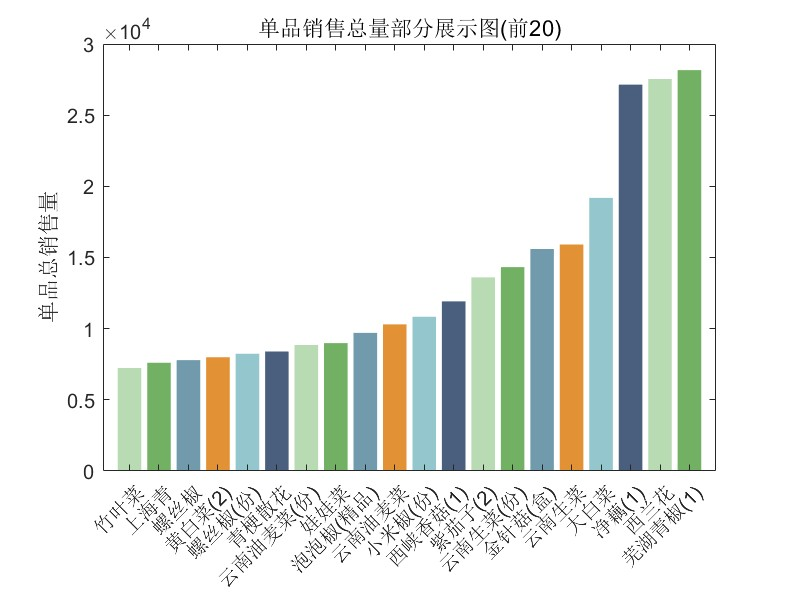
\includegraphics[width=14cm]{figures/picture_product_sale_part.jpg}
	\caption{ }\label{img001}
	\end{figure}

如图~\ref{img001}~展示了销售总量排名前二十的单品，可以说是商超中最为畅销的几种单品了。

为了揭露单品间的内在联系，该模型采用了系统聚类方法\textbf{中K-means++算法}对单品销售数据进行聚类。经过不断迭代优化，最终确定了三个聚类中心，如表~\ref{tab002}~所示，将单品划分成了四个部分，部分之间的单品主要因为受价格等因素而浮动的销售量所影响。

\begin{table}[!htbp]
	\caption{最终聚类中心}\label{tab002} \centering
	\begin{tabular}{cccc}
		\toprule[1.5pt]
		聚类中心 & 1 & 2 & 3  \\
		\midrule[1pt]
		
		销量（千克）& 588.281 & 25509.554 & 8140.738\\

		\bottomrule[1.5pt]
	\end{tabular}
\end{table}

\subsubsection{品类销售量分布和品类间关联性分析}

对于品类销售量的分布，我们通过excel对附加二的数据进行处理，得到三年里每种品类每天的销售量，即求出各品类销售量在时间上的分布，以分析不同品类销售量的变化趋势和季节性特征。
	
	\begin{figure}[h]
	\small
	\centering
	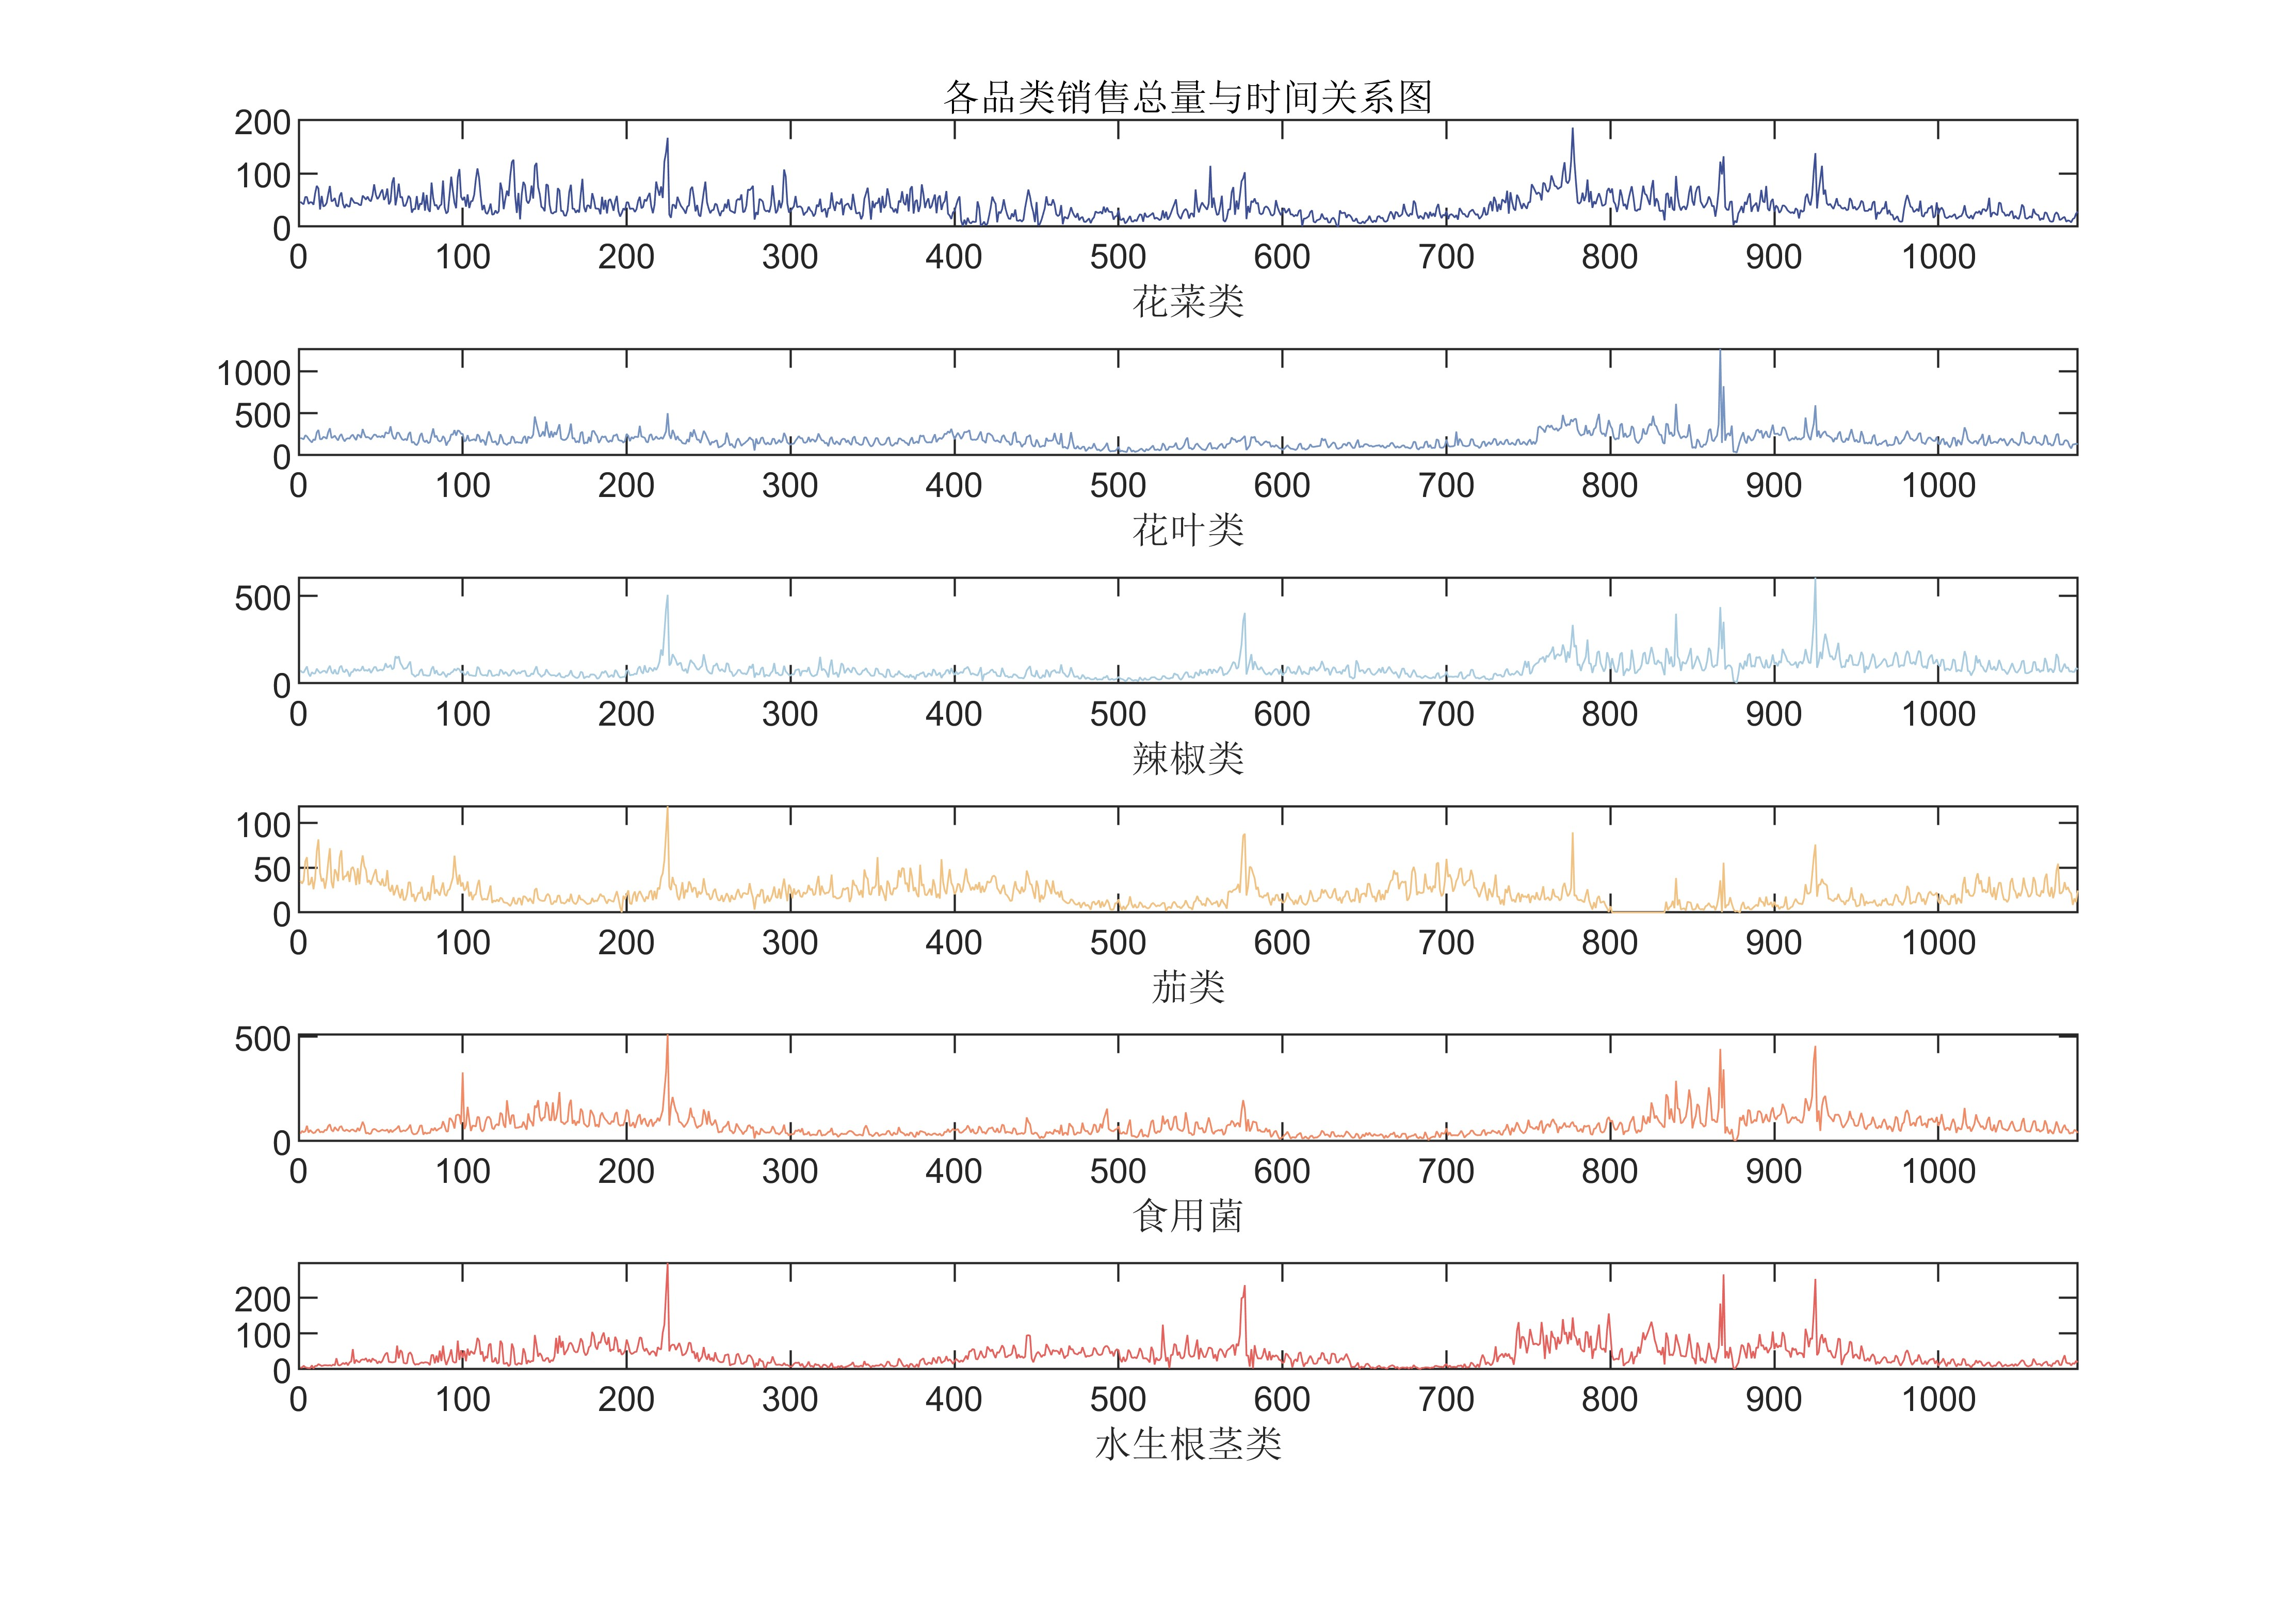
\includegraphics[width=13cm]{figures/picture_category_sale.jpg}
	\caption{ }\label{img002}
	\end{figure}

如图~\ref{img002}~所示，在深入剖析六类植物随时间推移的销量变化趋势时，一个显著的模式跃然纸上：绝大多数植物类别的销量呈现出鲜明的年度周期性波动，这一现象深刻反映了农业生产的自然规律——作物生长周期普遍遵循一年一度的节律，加之气候更迭与季节变换的周期性影响，共同塑造了市场需求与供应的年度波动图谱。

尤为值得注意的是，花叶类与花菜类植物在销量时间分布上的表现却显得尤为平稳与和缓，这一特征背后蕴含着多重原因。首先，花叶类植物往往因其观赏价值与美化环境的功效而备受青睐，其消费需求不仅局限于食用或特定季节，更融入了日常生活美学之中，从而削弱了季节更迭对销量的直接影响。其次，随着园艺文化的普及与生活品质的提升，消费者对于家庭绿植与花卉的需求日益增长，这种持续性的兴趣与需求支撑了花叶类植物销量的平稳发展。再者，花菜类植物，尽管其食用属性占据主导，但部分品种因其独特的营养价值、口感或文化寓意，也逐渐脱离了单一季节的限制，成为全年均可消费的食材，进而减缓了销量随季节波动的幅度。

为了分析品类间的关联性，我们先将每两类的销量作散点图进行直观上的分析，如图~\ref{img003}~所示，很明显，感觉两两种类作物之间的日销量并没有明显的线性关系。

	\begin{figure}[h]
	\small
	\centering
	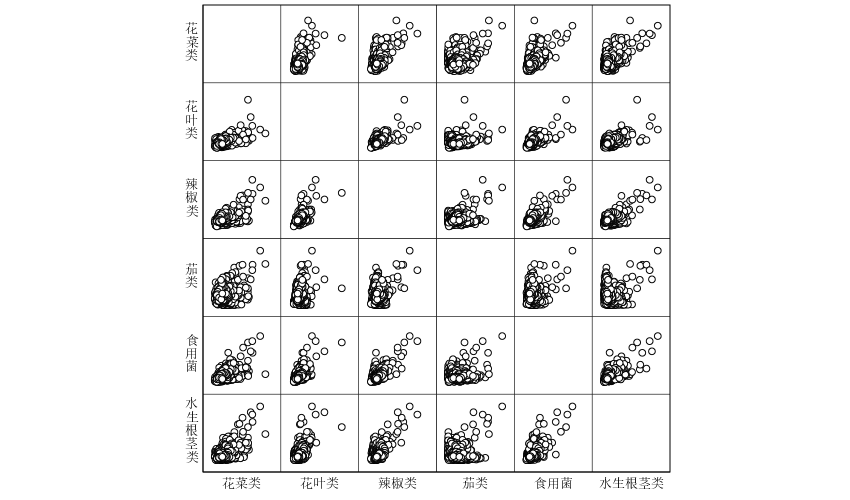
\includegraphics[width=13cm]{figures/散点图.png}
	\caption{ }\label{img003}
	\end{figure}

随后，我们针对每一种类植物的所有日销量数据实施了严谨的正态性分布检验。通过直观的\textbf{QQ图}，以花菜类图~\ref{img004}~为例观察，可以清晰地辨识出数据并不遵循正态分布的理想形态。
	
	\begin{figure}[h]
		\small
		\centering
		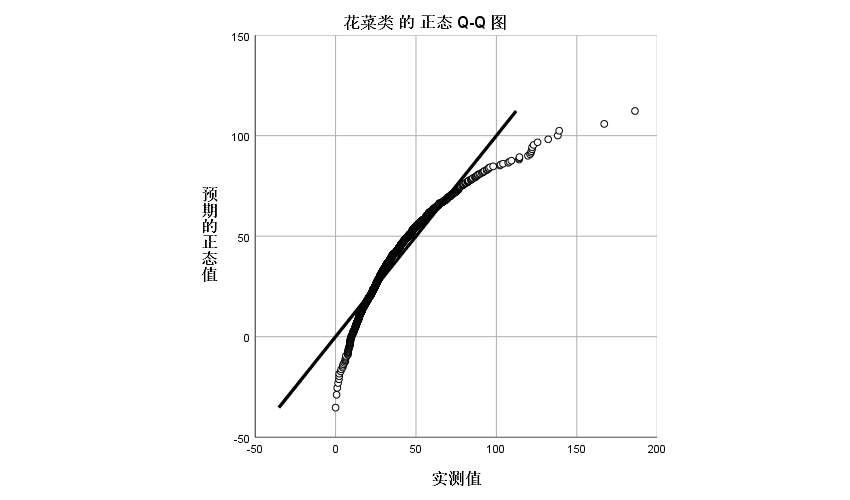
\includegraphics[width=13cm]{figures/花菜类.png}
		\caption{ }\label{img004}
	\end{figure}

进一步地，对于每个种类的日销量可以记为随机变量$X$，我们采用了定量的\textbf{JB检验}进行深入分析。

	\begin{equation}\label{equ001} 
		J B=\frac{n}{6}\left[S^2+\frac{(K-3)^2}{4}\right]
	\end{equation}

首先通过偏度$S$和峰度$K$,由公式~\ref{equ001}~构造出JB统计量,然后进行假设检验，发现每个种类计算出所对应的$p$值均小于0.05,故拒绝原假设。

该检验的结果同样明确地指出了这些销量数据并不满足正态分布的条件。

故而我们选择了\textbf{Spearman相关系数}，来分析两两品类间的相关性。
对于任取两组种类的日销量数据，分别记为$X_{i},Y_{i}$,其Spearman相关系数由公式~\ref{equ002}~可以计算得到。

\begin{equation}\label{equ002} 
	r_s=1-\frac{6 \sum_{i=1}^n d_i^2}{n\left(n^2-1\right)}
\end{equation}

其中，$d_{i}$为$X_i,Y_i$之间的等级差。
最终得到表~\ref{tab003}~。很明显，花叶类与花菜类的正相关性很强，水生根茎类和茄类的负相关性最强。茄类与辣椒类几乎没有相关性。

\begin{table}[!htbp]
	\caption{Spearman相关系数表}\label{tab003} \centering
	\begin{tabular}{|c|c|c|c|c|c|c|} 
		\toprule
		& 花菜类     & 花叶类     & 辣椒类     & 茄类       & 食用菌      & 水生根茎类     \\ 
		\hline
		花菜类   & 1.0000~ & 0.6334~ & 0.4296~ & 0.1929~  & 0.4624~  & 0.3956~   \\ 
		\hline
		花叶类   & 0.6334~ & 1.0000~ & 0.5949~ & 0.2522~  & 0.5964~  & 0.4389~   \\ 
		\hline
		辣椒类   & 0.4296~ & 0.5949~ & 1.0000~ & 0.1033~  & 0.5350~  & 0.3335~   \\ 
		\hline
		茄类    & 0.1929~ & 0.2522~ & 0.1033~ & 1.0000~  & -0.1144~ & -0.2099~  \\ 
		\hline
		食用菌   & 0.4624~ & 0.5964~ & 0.5350~ & -0.1144~ & 1.0000~  & 0.6048~   \\ 
		\hline
		水生根茎类 & 0.3956~ & 0.4389~ & 0.3335~ & -0.2099~ & 0.6048~  & 1.0000~   \\
		\bottomrule
	\end{tabular}
\end{table}

\subsection{问题二的模型建立与求解}
\subsubsection{模型建立思路}
\textbf{数据收集与预处理}：利用已有数据（附表二），计算每个品类每天的总销售量以及通过销售额加权平均得到的平均价格。并对对数据进行清洗，确保数据的准确性和完整性。

\textbf{价格-销售量关系模型构建}：针对每个品类，通过matlab编程，采用\textbf{指数回归}的曲线拟合方式，建立价格与销售量之间的数学关系模型。

\textbf{预测未来销售量与价格}：在预测模型方面，本文选择了在处理长期依赖关系的时间序列数据中预测效果较优异的LSTM神经网络架构。相对于传统的RNN架构，如NAR与NARX等神经网络模型，LSTM通过引入包括了输入门、遗忘门和输出门的门控机制与时间单元有效地解决了由于递归预测的误差累积引起的梯度消失与梯度爆炸等问题，避免了因神经网络的底层网络错误导致的训练模型难以收敛与不稳定等现象的发生。本项目所搭建的LSTM神经网络模型中，根据所需预测时间序列的单维数据特征，选择了利用预测值更新网络状态的方式。同时，在模型预测结果评价方面，本文选择RMSE值作为指标。基于详尽的历史销售数据和\textbf{LSTM预测}模型，我们预测了2023年7月1日至7日这一关键时间段内各类蔬菜的销售量。图~\ref{img005}~是花菜类销售量预测效果对比图。
\begin{figure}[h]
	\small
	\centering
	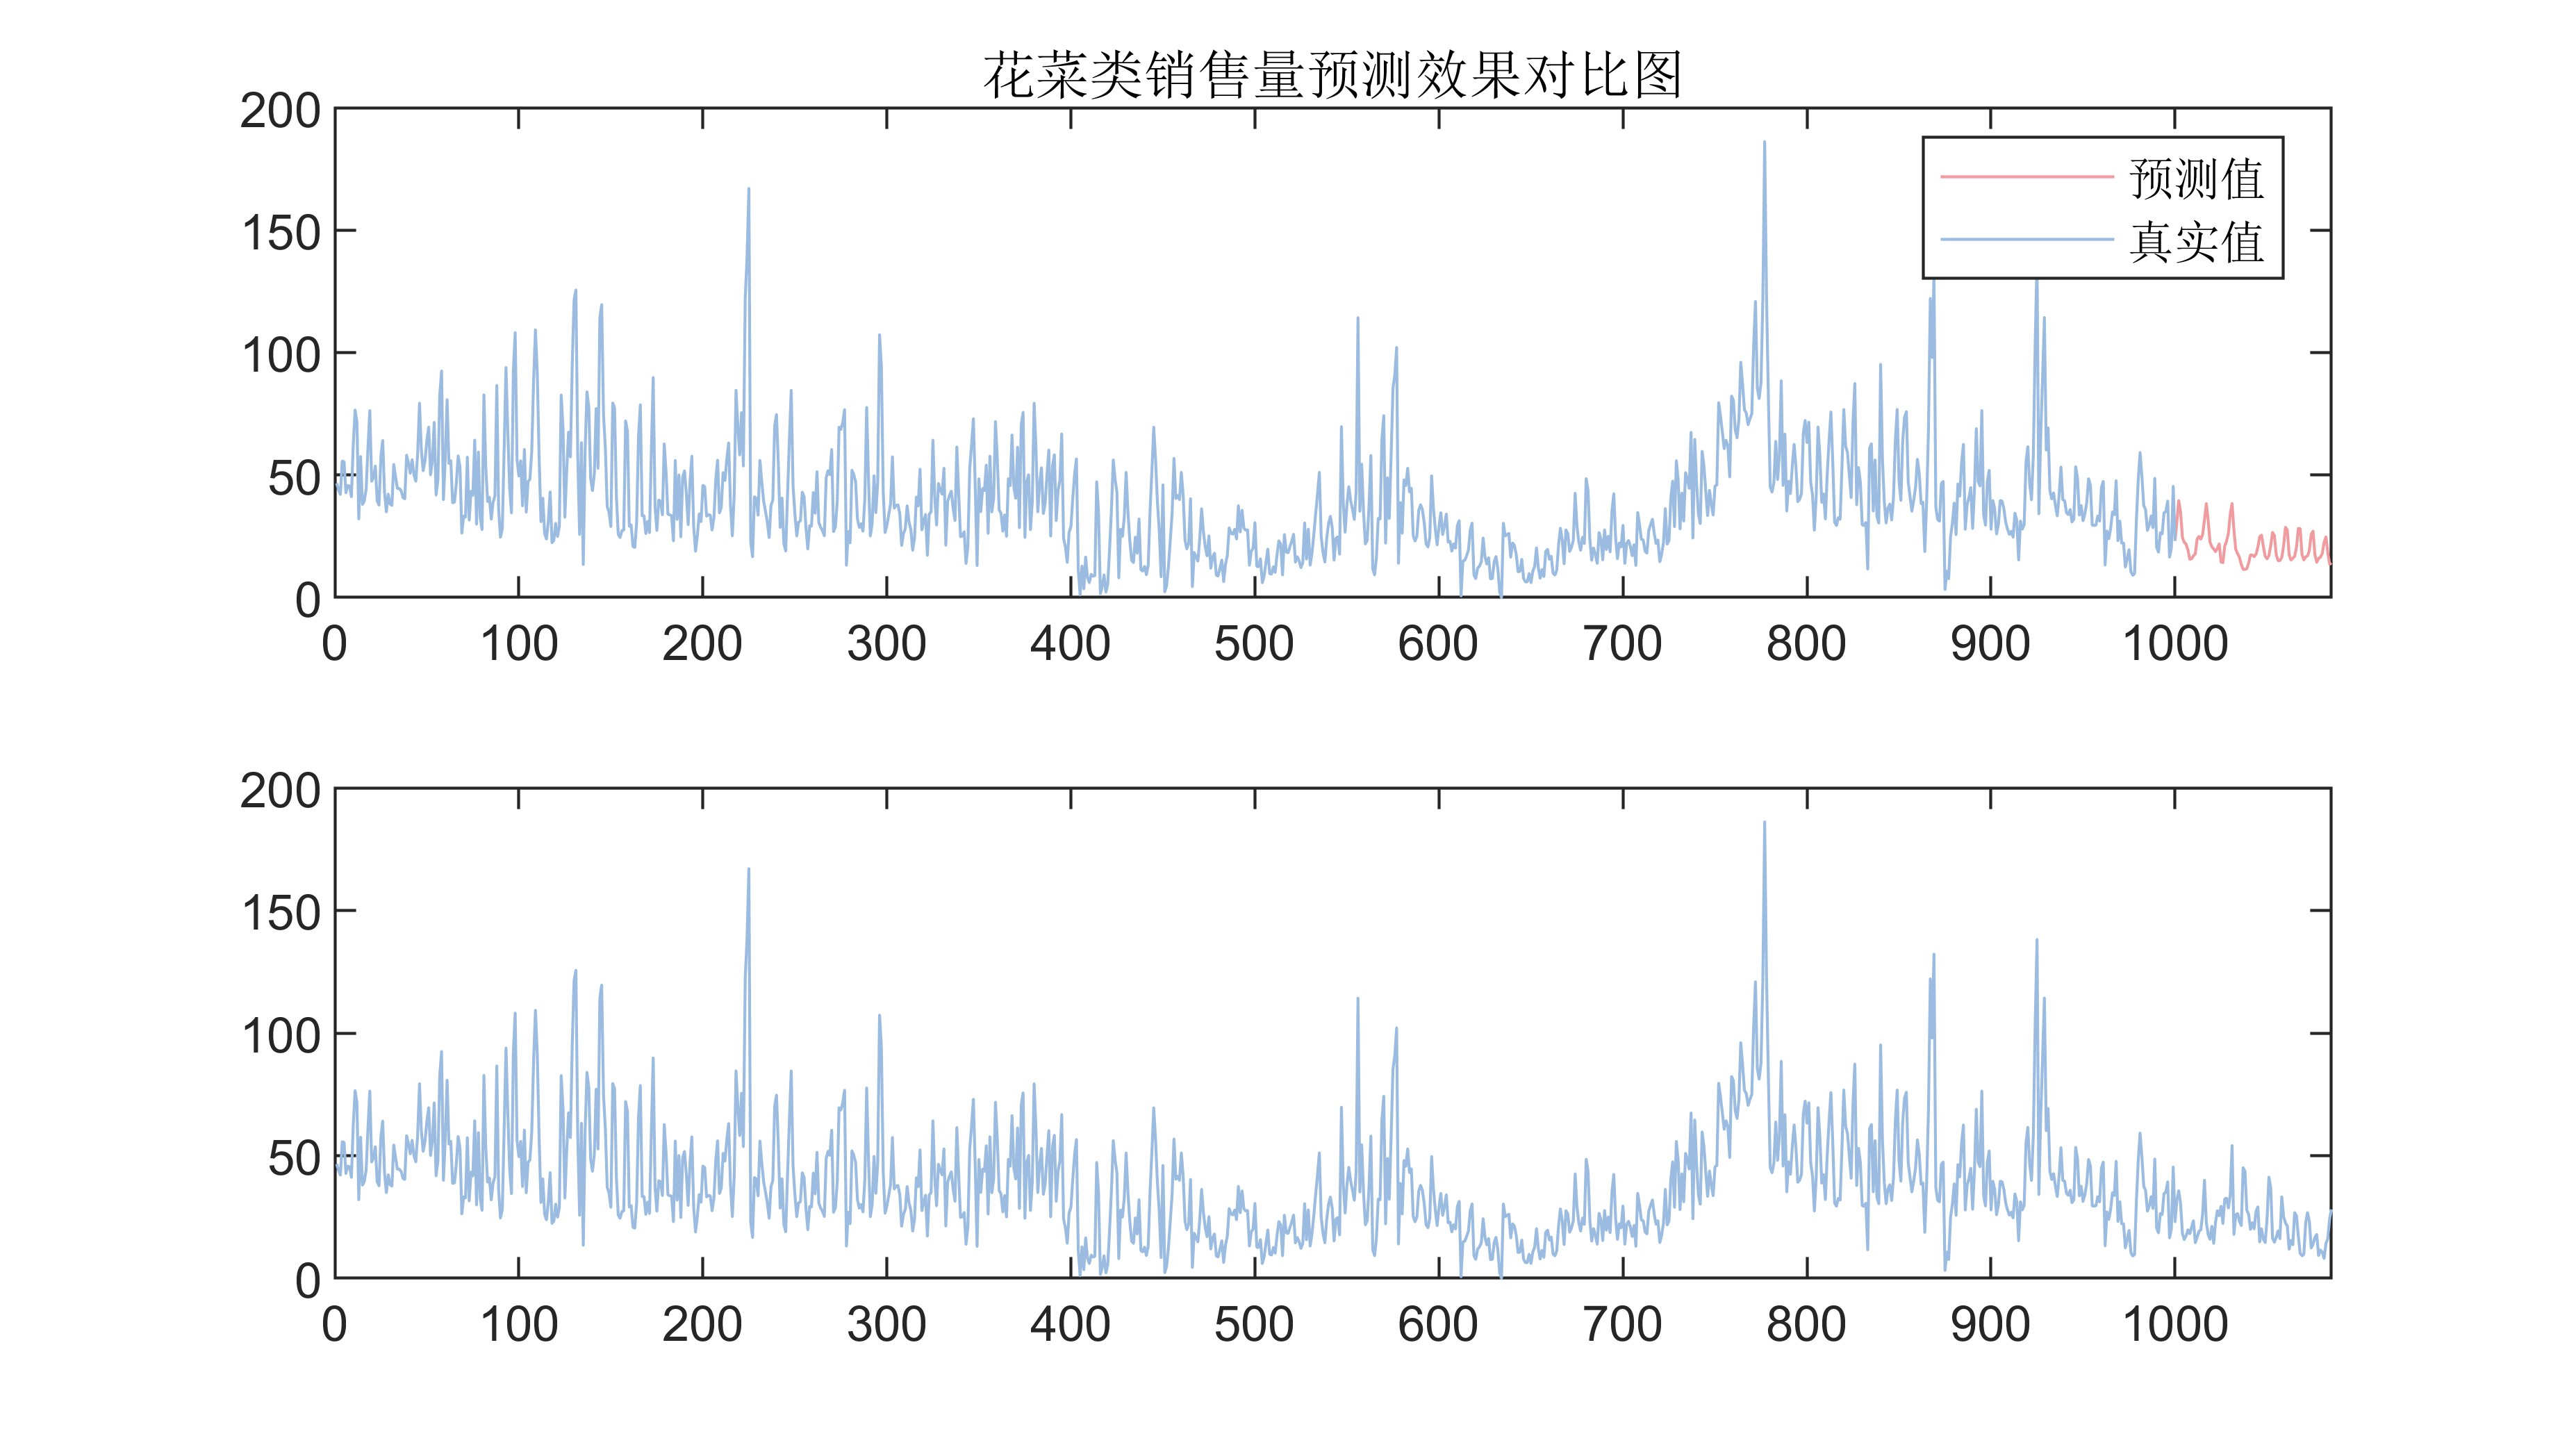
\includegraphics[width=15cm]{figures/花菜类预测.jpg}
	\caption{ }\label{img005}
\end{figure}

通过观察预测曲线与真实曲线的数据变化对比发现，预测结果与真实值在变化趋势与数据呈现上都十分接近。同时，根据上述公式计算得该模型预测结果与真实值的均方误差为9.93，数字较小，即模型预测结果逐渐接近真实值，预测精度也较高。

对于花菜类而言，所预测出这七天的销售量（保留两位小数，单位kg）依次是14.66，15.88，18.88，21.30，18.38，13.5，12.12。

随后，我们结合各品类的平均成本、损耗率等关键经济指标，以及前期通过深入统计分析构建的价格与销售量之间的数学关系模型，构建了一个综合的利润优化体系。在此基础上，我们利用LINGO这一专业的数学规划软件，对利润函数进行了精细的求解与优化，确保在供给量满足预测销售量的前提下，实现商超销售利润的最大化。最终，为商超制定了该时段内各类蔬菜的合理平均价格。
\subsubsection{模型求解}
对于六类蔬菜，日销量和均价的关系，最终拟合得到函数~\ref{equ003}~,从上到下依次是：花菜类，花叶类，辣椒类，茄类，食用菌，水生根茎类。
\begin{equation}\label{equ003}
	\begin{aligned}
		y & = -20.3lnx + 79.7\\
		y & = -52.3lnx + 270.7\\
		y & = -12.3lnx + 45.3\\
		y & = -41.0lnx + 167.0\\
		y & = -59.6lnx + 211.8\\
		y & = -30.0lnx + 102.5
	\end{aligned}
\end{equation}

接着通过LSTM预测得到2023年7月1日至7日这一时间段内各类蔬菜的销售量（附录）。

最后使用Lingo对该规划问题求出利润函数的最优解。

对于利润$z$来说,利润函数可以用公式~\ref{equ004}~来表示。

\begin{equation}\label{equ004} 
	\begin{split}
	z&=\sum_i \sum_j \text{Supply}_{i j}\left(1-\text { Damage }_i\right) \times\left(\text { Price } i j-\text { Capital }_i\right)\\
	&+\sum_i \sum_j \text {Supply}_{i j} \times \text { Damage }_i \times 80 \% \times\left(\text { Price }_{i j}-\text { Capital } i\right)
	\end{split}
\end{equation}

其中，供货量矩阵$\text{Supply}_{i j}$ 和定价矩阵$\text { Price } i j$满足函数~\ref{equ003}~ ,平均成本$\text { Capital }_i$由附件四可以计算得到，折损率 $\text { Damage }_i$ 从附件三中可以读取。同时，该利润矩阵还满足供货量小于等于预测销量。且80\%是指假定菜品折损后以八折出售。

通过Lingo求解最终得到，当花菜类，花叶类，辣椒类，茄类，食用菌，水生根茎类依次平均定价（元）为0.8，5.77,4.45,5.69,7.69,6.15,8.09时，商超将达到最大利润，最大利润为31266.85元。

\subsection{问题三的模型建立与求解}
\subsubsection{模型建立思路}
\textbf{数据处理}：处理附件二中的销售量数据，得到6.24-6.30售卖单品的销售量。成本是对附件四中的数据处理后得到平均成本。单价是对附件二的数据处理后得到的平均单价。损耗取自附件三中的相关数据。

\textbf{预测分析}：由于该问题属于短期预测，波动小，所以我们利用历史销售数据，采用\textbf{GM(1,1)灰色预测}预测方法，对如7月1日的单品销售量进行预测。

\textbf{遗传算法求解}：采用遗传算法等启发式搜索算法对补货量与定价问题进行求解。

\subsubsection{模型求解}
首先通过excel进行了数据处理，得到预测所需的相关数据。然后通过matlab软件进行灰色预测，得到了7.1日各种单品的销售量。

最终得到拟合函数式~\ref{equ005}~。预测7.1日单品销售量为11.3866kg。

\begin{equation}\label{equ005} 
	x_pro = 567.015-550.446e^{-0.0249405}t
\end{equation}


同时为了检验模型以单品编号102900005115786为例，在表~\ref{tab004}~展示预测相关信息。

\begin{equation}\label{equ006} 
	\varepsilon(k)=\frac{\left|x^{(0)}(k)-\hat{x}^{(0)}(k)\right|}{x^{(0)}(k)}
\end{equation}


其中，预测值的相对误差通过公式~\ref{equ006}~计算，由表~\ref{tab004}~中的计算结果可以看出相对误差都小于0.2，所以此题用灰色预测是符合条件的。

\begin{table}[!htbp]
	\caption{编号102900005115786单品销量相关预测信息}\label{tab004} \centering
	\begin{tabular}{|c|c|c|c|c|c|c|c|} 
		\toprule
		日期（2023年）     & 6.24     & 6.25     & 6.26       & 6.27      & 6.28  & 6.29  & 6.30  \\ 
		\hline
		真实值  & 16.569 & 13.941 & 12.022 & 14.095  & 13.151  & 10.415  & 12.884  \\ 
		\hline
		相对误差   & 0 & 0.027 & 0.100 & 0.085  & 0.043  & 0.178 & 0.071  \\ 
		
		\bottomrule
	\end{tabular}
\end{table}

然后采用遗传算法对补货量与定价问题按以下步骤进行求解。

\textbf{初始化种群}：我们首先用随机整数矩阵$Chose$来表示单品选择情况，并且保证单品选择数在$LimitMax$和$LimitMin$之间，即假定在27与33之间。然后初始化$Import$矩阵，根据$Chose$矩阵中的选择来决定每个单品的进口量，但确保不低于2.5。

\textbf{遗传算法迭代}：在每一代中，首先通过公式~\ref{equ007}~计算每个个体的适应度$fit$，这里通过计算考虑损耗和折扣后的总利润来定义。选出当前代中的最优个体$fBest_Chose$ 和 $fBest_Import$。通过轮盘赌选择来生成下一代种群的一部分。然后在交叉概率$Pc$ 下对选中的个体进行交叉操作，随机选择两个个体并交换它们的部分基因（我们选择是产品选择和进口量）。在变异概率 $Pv$ 下对所有个体进行变异操作，随机改变部分基因的值（这里是产品选择和进口量）。将最优个体直接复制到下一代中，以确保算法的收敛性。

\begin{equation}\label{equ007} 
	fit=(1-Damage)*Import*(Prize-Capital)+Damage*Discount*Import*(Prize-Capital)
\end{equation}

最终得到最优的产品选择 $fBest_Chose$ ，最优的进口量 $fBest_Import$（图~\ref{img006}~）和最优利润$maxfit$为749.61元。

\begin{figure}[h]
	\small
	\centering
	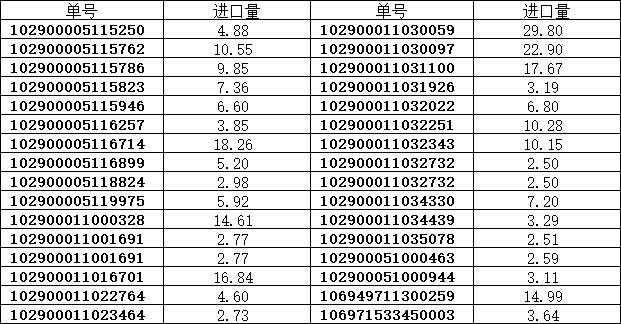
\includegraphics[width=15cm]{figures/最终单品选择.png}
	\caption{ }\label{img006}
\end{figure}

7月1日可售单品数为34，算法中将单品的成本简化为历史平均成本，损耗率参考附录4数据，损耗部分的折扣相同，算法中取0.8。

\subsection{问题四的求解与分析}
在优化生鲜商超蔬菜商品的补货和定价决策过程中，除了现有的销售、价格和损耗数据外，进一步采集以下几类相关数据将显著提升决策的精准度和有效性。以下是对所需数据及其重要性的分析：
\subsubsection{深化顾客需求洞察}

商超应加强对顾客购买行为、偏好及满意度的数据收集与分析。通过实时监控系统记录顾客购买数据，利用时间序列分析和聚类分析等方法，预测销售趋势并识别顾客群体特征。同时，开展定期的顾客满意度调查，收集顾客对蔬菜品质、价格及服务的反馈，以顾客需求为导向，不断优化商品结构和服务体验。

\subsubsection{强化供应链与物流管理}

建立完善的供应链与物流数据管理体系，包括供应商评估、冷链物流监控等关键环节。通过收集供应商交货准时率、质量评价等数据，评估供应商绩效，确保蔬菜供应的稳定性和可靠性。同时，利用冷链物流监控数据，保障蔬菜在运输和储存过程中的品质安全，减少损耗。此外，运用库存仿真等数模方法，优化补货策略，提高库存周转率，降低库存成本。

\subsubsection{灵活应对市场竞争}

商超应密切关注市场竞争动态，包括竞争对手的价格策略、促销活动及市场价格波动等。通过定期监测竞争对手数据，运用竞争分析模型评估自身市场地位，制定差异化的定价和促销策略。同时，建立灵活的价格调整机制，根据市场价格波动和顾客需求变化，及时调整采购成本和零售价格，保持市场竞争力。此外，利用价格敏感度分析等数模方法，评估价格变动对销售量的影响，为定价决策提供科学依据。

\section{结果分析与模型评价}
\subsection{模型检验及可靠性分析}
\subsubsection{模型检验}

\textbf{数据验证}：首先，我们对输入模型的历史销售数据进行了严格的验证，确保数据的准确性、完整性和一致性。通过对比不同来源的数据（如收银系统、库存管理系统等），我们排除了潜在的数据错误和异常值，确保模型输入数据的质量。

\textbf{模型拟合度检验}：对于使用曲拟合技术建立的销售量与平均价格之间的关系函数，我们进行了拟合度检验。通过计算残差平方和、决定系数（R²）等指标，我们评估了模型的拟合效果。结果显示，模型具有较高的拟合度，能够较好地反映销售量与价格之间的实际关系。

\textbf{预测准确性验证}：为了验证预测模型的准确性，我们将预测结果与后续实际销售数据进行了对比。通过计算预测误差率、均方误差（MSE）等指标，我们评估了预测模型的精度。结果显示，预测模型在多数情况下能够准确预测销售量，为补货与定价策略的制定提供了可靠依据。

\textbf{敏感性分析}：为了评估模型对参数变化的敏感性，我们进行了敏感性分析。通过调整关键参数（如成本、损耗率、价格上下限等），我们观察了模型输出结果的变化情况。结果显示，模型对参数变化具有一定的鲁棒性，能够在一定范围内保持稳定的输出结果。

\subsubsection{可靠性分析}

\textbf{算法稳定性}：我们选择的遗传算法等启发式搜索算法具有全局搜索能力强、鲁棒性好的优点。通过多次运行算法并观察结果的一致性，我们验证了算法的稳定性。结果显示，算法在多次运行中均能找到较为接近的最优解，证明了其可靠性。

\textbf{数据依赖性分析}：我们分析了模型对数据的依赖程度，并评估了数据质量对模型输出结果的影响。结果显示，模型对数据质量有一定的容忍度，但在数据质量较差的情况下，模型输出结果可能会出现较大偏差。因此，我们强调了数据治理的重要性，以确保模型输入数据的质量。

\textbf{约束条件合理性}：我们对模型中的约束条件进行了合理性分析。通过对比实际运营情况与约束条件设置，我们验证了约束条件的合理性和有效性。结果显示，约束条件能够较好地反映实际运营中的限制条件，为模型求解提供了有力的支持。

\subsection{模型评价与推广}
\subsubsection{模型优点}
\textbf{实用性}：本模型针对生鲜商超的运营需求，提供了科学的补货量与定价策略，显著提升了运营效率与盈利能力。然而，在实际应用中，商超仍需根据自身具体情况对模型进行适当调整，以确保其完全贴合实际运营需求。

\textbf{准确性}：模型在数据验证、拟合度检验及预测准确性方面表现良好，但也存在一定的局限性。例如，当销售数据受到异常事件（如天气突变、疫情等）影响时，模型的预测准确性可能会受到一定影响。因此，在实际应用中，商超需要密切关注市场动态，及时调整模型参数，以提高预测准确性。

\textbf{灵活性}：模型具有较高的灵活性，可根据商超的实际需求进行调整。但同时，这也对商超的数据分析和运营能力提出了较高要求。商超需要拥有专业的数据分析团队和先进的数据分析工具，以支持模型的持续优化和迭代。

\subsubsection{缺陷与改进}

\textbf{数据依赖性}：模型对数据质量要求较高，若数据存在缺失、错误或异常值，将直接影响模型的准确性和可靠性。因此，建议商超加强数据治理工作，建立完善的数据质量控制体系，确保数据的准确性和完整性。

\textbf{预测精度限制}：由于市场环境的复杂性和不确定性，模型在预测精度上仍存在一定的局限性。为提高预测精度，可以考虑引入更多的数据源（如社交媒体数据、天气预报等）和更先进的预测算法（如深度学习等），以丰富模型的信息输入和算法能力。

\textbf{约束条件灵活性}：模型中的约束条件是基于当前运营情况设定的，但未来随着商超的发展和市场环境的变化，这些约束条件可能需要进行调整。因此，建议商超定期评估模型约束条件的合理性，并根据实际情况进行必要的调整和优化。

\subsubsection{模型推广}
在克服了上述缺陷并进行了相应的改进后，本模型具有较高的推广价值。一方面，它可以应用于其他零售行业和供应链管理领域，通过调整模型参数和约束条件来适应不同行业的运营特点和需求；另一方面，通过技术升级和合作共享等方式，可以进一步提升模型的智能化水平和预测准确性，为相关企业提供更加精准的决策支持。同时，我们也鼓励商超之间加强合作与交流，共同推动零售行业的数字化转型和智能化升级。


\newpage
%附录

\begin{appendices}
\section{问题一相关代码和处理结果}
\subsection{单品分布规律绘图--matlab 源程序}
\begin{lstlisting}[language=matlab]
	x=["竹叶菜","上海青","螺丝椒","黄白菜(2)","螺丝椒(份)","青梗散花","云南油麦菜(份)","娃娃菜",
	"泡泡椒(精品)","云南油麦菜","小米椒(份)","西峡香菇(1)","紫茄子(2)","云南生菜(份)","金针菇(盒)",
	"云南生菜","大白菜","净藕(1)","西兰花","芜湖青椒(1)"]';
	colors=[184 219 179;114 176 99;113 154 172;226 145 53;148 198 205;
	74 95 126;184 219 179;114 176 99;113 154 172;226 145 53;
	148 198 205;74 95 126;184 219 179;114 176 99;113 154 172;
	226 145 53;148 198 205;74 95 126;184 219 179;114 176 99]./255;
	picture=bar(x,product_sale,'EdgeColor','none');
	picture.FaceColor="flat";
	for i=1:20
	picture.CData(i,:)=colors(i,:);
	end
	ylabel("单品总销售量")
	title("单品销售总量部分展示图(前20)")
\end{lstlisting}

\subsection{品类分布规律绘图--matlab 源程序}
\begin{lstlisting}[language=matlab]
	subplot(6,1,1);
	plot(huacai,Color=[62 79 148]./255,LineWidth=0.4)
	xlim([0,1085])
	xlabel("花菜类")
	title("各品类销售总量与时间关系图")
	set(gac,'Ylim')
	subplot(6,1,2);
	plot(huaye,Color=[120 149 193]./255,LineWidth=0.4)
	xlim([0,1085])
	xlabel("花叶类")
	subplot(6,1,3);
	plot(lajiao,Color=[168 203 223]./255,LineWidth=0.4)
	xlim([0,1085])
	xlabel("辣椒类")
	subplot(6,1,4);
	plot(qie,Color=[240 194 132]./255,LineWidth=0.4)
	xlim([0,1085])
	xlabel("茄类")
	subplot(6,1,5);
	plot(shiyongjun,Color=[239 139 103]./255,LineWidth=0.4)
	xlim([0,1085])
	xlabel("食用菌")
	subplot(6,1,6);
	plot(shuisheng,Color=[227 98 93]./255,LineWidth=0.4)
	xlim([0,1085])
	xlabel("水生根茎类")
	hold off
	xlim([0,1085])
	lables={"花菜类","花叶类","辣椒类","茄类","食用菌","水生根茎类"};
\end{lstlisting}
	
\subsection{品类之间相互关系JB检验--matlab 源程序}
\begin{lstlisting}[language=matlab]
	%JB正态分布检验
	clear,clc
	load Types.mat
	% 正态分布检验
	% 用循环检验所有列的数据
	a = size(Types,2);% number of column 数据的列数
	H = zeros(1,6);
	P = zeros(1,6);
	for i = 1:a
	[h,p] = jbtest(Types(:,i),0.05);
	H(i)=h;
	P(i)=p;
	end
	disp(H)
	disp(P)	
\end{lstlisting}

\subsection{各品类日销售量正态检验之QQ图}
\begin{figure}[!htb]
	\centering
	\subfloat{
		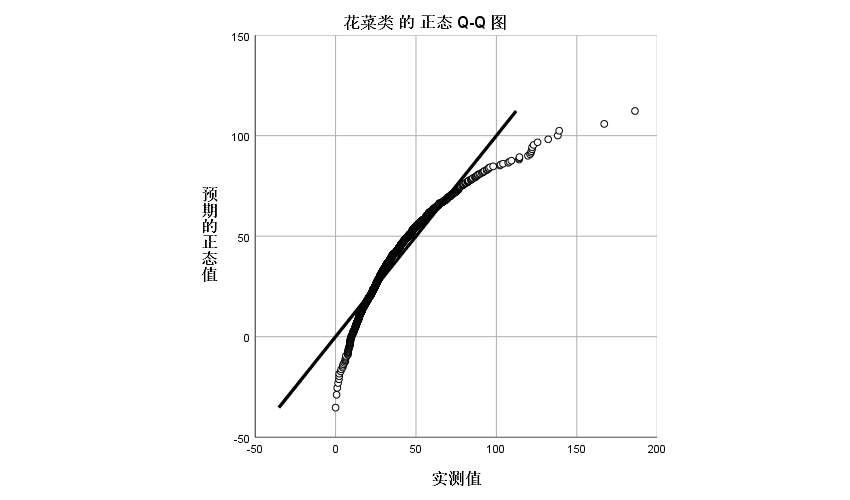
\includegraphics[width=4.5cm]{figures/花菜类.png}
	}
	\subfloat
	{
		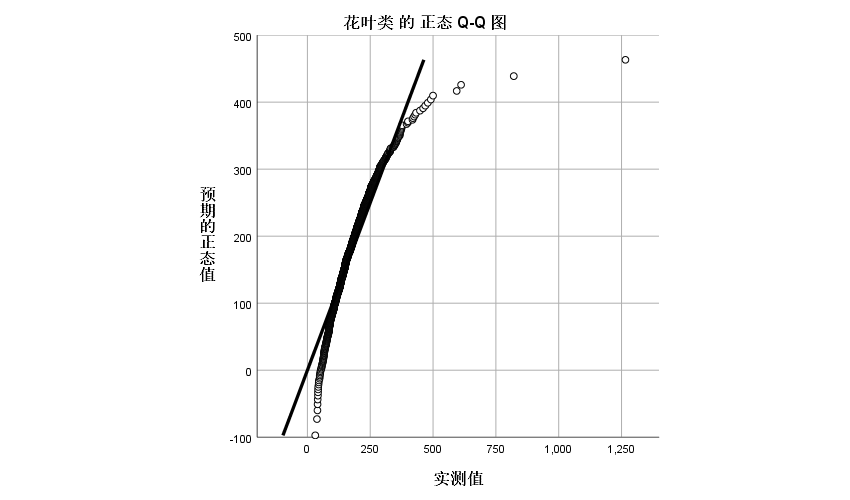
\includegraphics[width=4.5cm]{figures/花叶类.png}
	}
	\subfloat
	{
		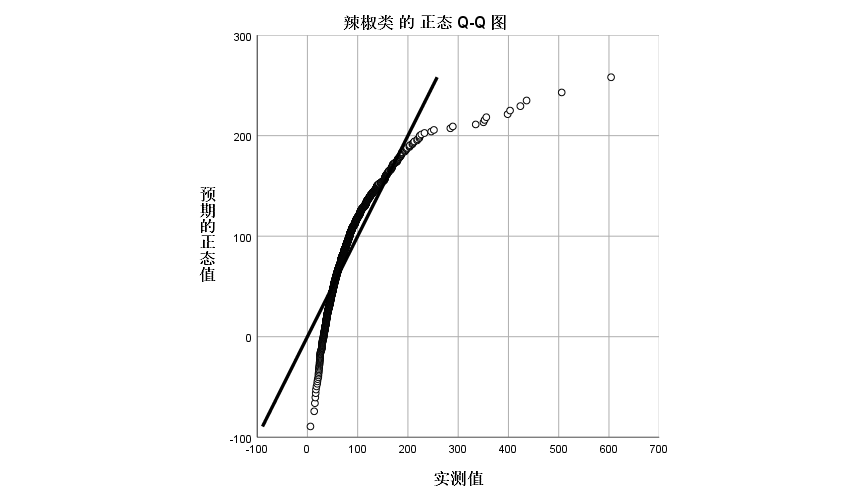
\includegraphics[width=4.5cm]{figures/辣椒类.png}
	}
	
	\subfloat{
		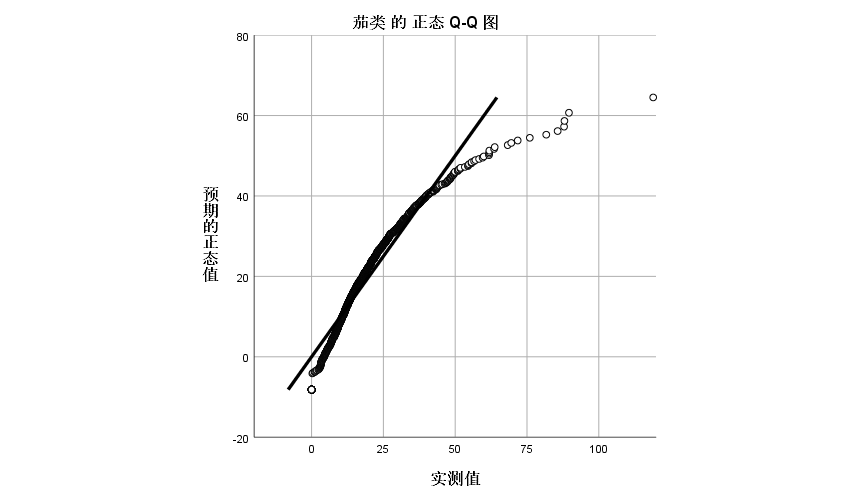
\includegraphics[width=4.5cm]{figures/茄类.png}
	}
	\subfloat
	{
		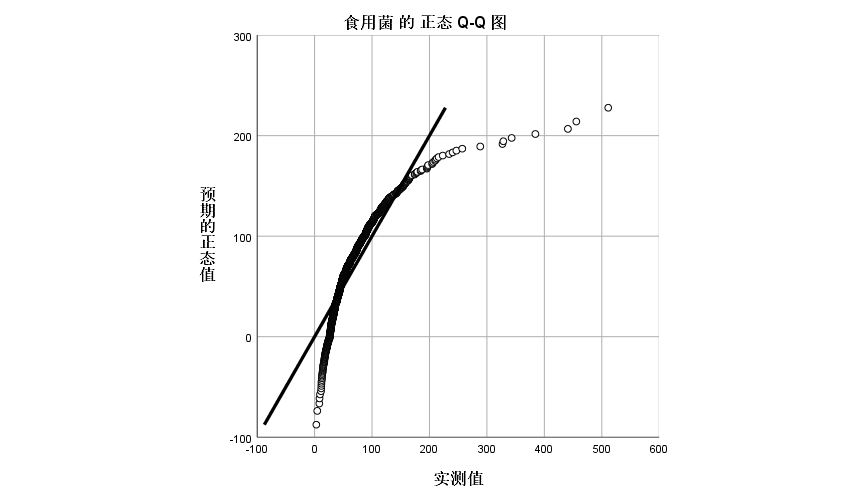
\includegraphics[width=4.5cm]{figures/食用菌.png}
	}
	\subfloat
	{
		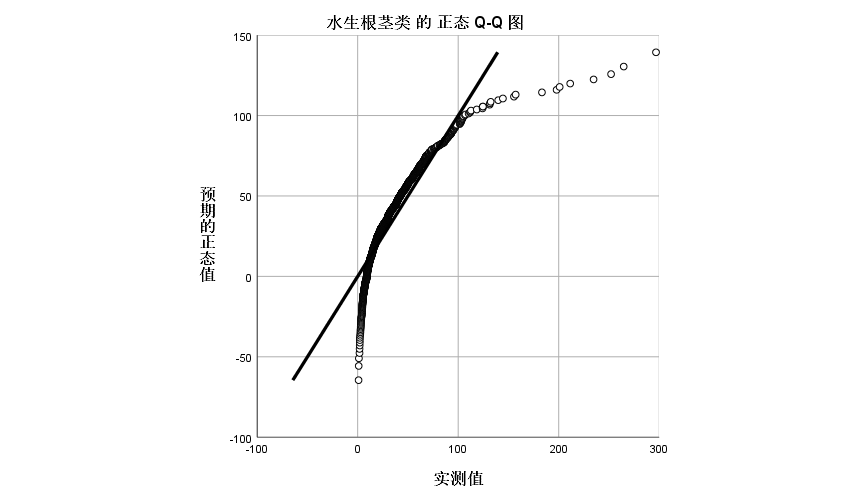
\includegraphics[width=4.5cm]{figures/水生根经类.png}
	}
\end{figure}

\subsection{品类之间Spearman相关系数计算--matlab 源程序}
\begin{lstlisting}[language=matlab]
	%spearman相关系数计算
	clear,clc
	load Types.mat
	[R,P]=corr(Types,'type','Spearman')
\end{lstlisting}

\subsection{品类之间Spearman相关系数表P检验值}
\begin{table}[!htb]
	\centering
	\begin{tabular}{|c|c|c|c|c|c|c|} 
		\toprule
		& 花菜类     & 花叶类     & 辣椒类     & 茄类      & 食用菌     & 水生根茎类    \\ 
		\hline
		花菜类   & 1.0000~ & 0.0000~ & 0.0000~ & 0.0000~ & 0.0000~ & 0.0000~  \\ 
		\hline
		花叶类   & 0.0000~ & 1.0000~ & 0.0000~ & 0.0000~ & 0.0000~ & 0.0000~  \\ 
		\hline
		辣椒类   & 0.0000~ & 0.0000~ & 1.0000~ & 0.0007~ & 0.0000~ & 0.0000~  \\ 
		\hline
		茄类    & 0.0000~ & 0.0000~ & 0.0007~ & 1.0000~ & 0.0002~ & 0.0000~  \\ 
		\hline
		食用菌   & 0.0000~ & 0.0000~ & 0.0000~ & 0.0002~ & 1.0000~ & 0.0000~  \\ 
		\hline
		水生根茎类 & 0.0000~ & 0.0000~ & 0.0000~ & 0.0000~ & 0.0000~ & 1.0000~  \\
		\bottomrule
	\end{tabular}
\end{table}

\section{问题二相关代码和处理结果}

\subsection{定价与销售量曲线拟合--matlab 源程序}
\begin{lstlisting}[language=matlab]
	clear,clc
	load wash_Types.mat
	load wash_Types_Price.mat
	
	huacai=wash_Types(:,1);
	huaye=wash_Types(:,2);
	lajiao=wash_Types(:,3);
	qie=wash_Types(:,4);
	shiyongjun=wash_Types(:,5);
	genjing=wash_Types(:,6);
	
	huacai_Price=wash_Type_Price(:,1);
	huaye_Price=wash_Type_Price(:,2);
	lajiao_Price=wash_Type_Price(:,3);
	qie_Price=wash_Type_Price(:,4);
	shiyongjun_Price=wash_Type_Price(:,5);
	genjing_Price=wash_Type_Price(:,6);
	
	%% 拟合: '根茎类'。
	[xData, yData] = prepareCurveData( genjing_Price, genjing );
	
	% 设置 fittype 和选项。
	ft = fittype( 'log' );
	
	% 对数据进行模型拟合。
	[fitresult, gof] = fit( xData, yData, ft );
	
	% 绘制数据拟合图。
	figure( 'Name', '根茎类' );
	h = plot( fitresult, xData, yData );
	legend( h, 'genjing vs. genjing_Price', '根茎类', 'Location', 'NorthEast', 'Interpreter', 'none' );
	% 为坐标区加标签
	xlabel( 'genjing_Price', 'Interpreter', 'none' );
	ylabel( 'genjing', 'Interpreter', 'none' );
	grid on
	
	%% 拟合: '花叶类'。
	[xData, yData] = prepareCurveData( huaye_Price, huaye );
	
	% 设置 fittype 和选项。
	ft = fittype( 'log' );
	
	% 对数据进行模型拟合。
	[fitresult, gof] = fit( xData, yData, ft );
	
	% 绘制数据拟合图。
	figure( 'Name', '花叶类' );
	h = plot( fitresult, xData, yData );
	legend( h, 'huaye vs. huaye_Price', '花叶类', 'Location', 'NorthEast', 'Interpreter', 'none' );
	% 为坐标区加标签
	xlabel( 'huaye_Price', 'Interpreter', 'none' );
	ylabel( 'huaye', 'Interpreter', 'none' );
	grid on
	
	%% 拟合: '食用菌'。
	[xData, yData] = prepareCurveData( shiyongjun_Price, shiyongjun );
	
	% 设置 fittype 和选项。
	ft = fittype( 'log' );
	
	% 对数据进行模型拟合。
	[fitresult, gof] = fit( xData, yData, ft );
	
	% 绘制数据拟合图。
	figure( 'Name', '食用菌' );
	h = plot( fitresult, xData, yData );
	legend( h, 'shiyongjun vs. shiyongjun_Price', '食用菌', 'Location', 'NorthEast', 'Interpreter', 'none' );
	% 为坐标区加标签
	xlabel( 'shiyongjun_Price', 'Interpreter', 'none' );
	ylabel( 'shiyongjun', 'Interpreter', 'none' );
	grid on
	
	%% 拟合: '茄类'。
	[xData, yData] = prepareCurveData( qie_Price, qie );
	
	% 设置 fittype 和选项。
	ft = fittype( 'log' );
	excludedPoints = excludedata( xData, yData, 'Indices', [12 13 23 28 29 33 34 46 68 82 95 96 98 197 219 221 222 223 224 225 226 228 229 230 234 317 325 424 445 529 572 573 579 580 581 582 583 585 645 669 670 679 680 681 687 702 716 730 799 801 802 803 804 805 806 807 808 809 810 811 812 813 814 815 816 817 818 819 820 821 822 823 824 825 826 827 828 829 830 831 832 833 868 878 879 919 923 924 927 928 929 930 931 932 981 1024 1066] );
	opts = fitoptions( 'Method', 'LinearLeastSquares' );
	opts.Exclude = excludedPoints;
	
	% 对数据进行模型拟合。
	[fitresult, gof] = fit( xData, yData, ft, opts );
	
	% 绘制数据拟合图。
	figure( 'Name', '茄类' );
	h = plot( fitresult, xData, yData, excludedPoints );
	legend( h, 'qie vs. qie_Price', '已排除 qie vs. qie_Price', '茄类', 'Location', 'NorthEast', 'Interpreter', 'none' );
	% 为坐标区加标签
	xlabel( 'qie_Price', 'Interpreter', 'none' );
	ylabel( 'qie', 'Interpreter', 'none' );
	grid on
	
	%% 拟合: '花菜类'。
	[xData, yData] = prepareCurveData( huacai_Price, huacai );
	
	% 设置 fittype 和选项。
	ft = fittype( 'log' );
	excludedPoints = excludedata( xData, yData, 'Indices', [4 5 11 19 26 40 42 46 72 92 93 94 101 103 135 138 142 146 151 152 166 208 221 240 277 289 374 380 752 765 766 767 770 788 792 793 794 798 799 800 801 807 813 820 849 854 875 876 877 895] );
	opts = fitoptions( 'Method', 'LinearLeastSquares' );
	opts.Exclude = excludedPoints;
	
	% 对数据进行模型拟合。
	[fitresult, gof] = fit( xData, yData, ft, opts );
	
	% 绘制数据拟合图。
	figure( 'Name', '花菜类' );
	h = plot( fitresult, xData, yData, excludedPoints );
	legend( h, 'huacai vs. huacai_Price', '已排除 huacai vs. huacai_Price', '花菜类', 'Location', 'NorthEast', 'Interpreter', 'none' );
	% 为坐标区加标签
	xlabel( 'huacai_Price', 'Interpreter', 'none' );
	ylabel( 'huacai', 'Interpreter', 'none' );
	grid on
	
	%% 拟合: '辣椒类'。
	[xData, yData] = prepareCurveData( lajiao_Price, lajiao );
	
	% 设置 fittype 和选项。
	ft = fittype( 'log' );
	excludedPoints = excludedata( xData, yData, 'Indices', [159 160 161 165 167 168 169 170 171 172 173 174 175 176 177 178 179 180 181 182 183 184 185 186 187 188 189 190 191 192 193 194 195 196 197 198 199 200 201 202 203 204 205 206 207 208 209 210 211 212 213 214 215 216 217 218 219 220 221 222 223 224 225 226 227 228 229 230 231 232 233 234 573 574 575 576 577 578 579 580 581 582 583 584 585 586 611 625 626 627 628 629 630 631 632 633 635 636 638 641 642] );
	opts = fitoptions( 'Method', 'LinearLeastSquares' );
	opts.Exclude = excludedPoints;
	
	% 对数据进行模型拟合。
	[fitresult, gof] = fit( xData, yData, ft, opts );
	
	% 绘制数据拟合图。
	figure( 'Name', '辣椒类' );
	h = plot( fitresult, xData, yData, excludedPoints );
	legend( h, 'lajiao vs. lajiao_Price', '已排除 lajiao vs. lajiao_Price', '辣椒类', 'Location', 'NorthEast', 'Interpreter', 'none' );
	% 为坐标区加标签
	xlabel( 'lajiao_Price', 'Interpreter', 'none' );
	ylabel( 'lajiao', 'Interpreter', 'none' );
	grid on
	
\end{lstlisting}

\subsection{品类销售量LSTM预测--matlab 源程序}
\begin{lstlisting}[language=matlab]
clc
clear
load matlab.mat
data=huacai;
data=data(:,1)';  %设置数据格式
dataTrain = data(1:1000);   %训练集
dataTest = data(1001:end);    %测试集

mu = mean(dataTrain);    
sig = std(dataTrain);    
dataTrainStandardized = (dataTrain - mu) / sig;    %标准化训练集数据
XTrain = dataTrainStandardized(1:end-1);     %设置预测步数为1
YTrain = dataTrainStandardized(2:end);  
numFeatures = 1;    %设置为单维单步时间序列分段
numResponses = 1;  
numHiddenUnits = 40;  %设置LSTM隐含层为200

layers = [ ...
sequenceInputLayer(numFeatures)     %输入层   
lstmLayer(numHiddenUnits)   %LSTM层
fullyConnectedLayer(numResponses)   %全连接层  
regressionLayer];     %计算均方误差
options = trainingOptions('adam', ...   %解释器
'MaxEpochs',600, ...   %进行1000轮训练
'GradientThreshold',1, ...  %设置梯度阈值
'InitialLearnRate',0.15, ...      %设置初始学习率
'LearnRateSchedule','piecewise', ...?
%表示经过一定数量时期学习率就会乘一个系数以降低学习率
'LearnRateDropPeriod',150, ...      
'LearnRateDropFactor',0.08, ...      
'Verbose',0,  ...  
'Plots','training-progress');   
net = trainNetwork(XTrain,YTrain,layers,options); 
net = predictAndUpdateState(net,XTrain);  %初始化网络状态
[net,YPred] = predictAndUpdateState(net,YTrain(end));  
%利用预测值更新网络状态
for i = 2:95
[net,YPred(:,i)] = predictAndUpdateState(net,YPred(:,i-1), ...
'ExecutionEnvironment','cpu'); 
%利用前一个值预测后一个值，预测结果写入YPred
end

YPred = sig*YPred + mu;      %对预测值去标准化
rmse = sqrt(mean((YPred(1:85)-dataTest).^2)) ;   
%预测值与真实值计算均方根误差 
disp(rmse);
subplot(2,1,1)
plot(dataTrain(1:end))   
hold on
idx = 1001:1095;  
plot(idx,YPred(1:95),'.-') 
hold on 
plot([1000,1001],[dataTrain(end),YPred(1)])
hold off
xlabel("Time")
ylabel("Case")
title("Forecast")
legend(["Observed" "Forecast"])
subplot(2,1,2)
plot(data)
xlabel("Time")
ylabel("Case")
title("Dataset")
figure(2)
idx = 1001:1095;  
plot(idx,YPred(1:95),'.-')  
hold off
\end{lstlisting}

 \subsection{品类决策规划解决程序--lingo源代码}
\begin{lstlisting}[language=c]
	sets:
	Types/1..6/:Capital,Damage;
	day/1..7/;
	joint(Types,day):Willsold,Supply,Price;
	end sets
	
	data:
	s=0.8;
	Willsold=
	14.664984	102.06803	70.964966	36.401798	45.353745	24.036121	
	15.877178	140.93683	151.60938	32.409264	70.191841	19.551228	
	18.878981	164.649	263.56628	15.613374	74.514755	18.2339	
	21.298077	93.384529	178.22588	27.18099	40.250347	18.903116	
	18.378319	78.628639	102.56927	14.736989	47.848621	21.299776	
	13.492289	152.2863	76.54847	34.937481	43.711452	27.743694	
	12.117132	155.05222	109.69466	38.334759	48.172028	29.136339	
	;
	Damage=0.1414,0.01028,0.0712,0.0852,0.0813,0.1197;
	Capital=5.77,4.45,5.69,7.69,6.15,8.09;
	end data
	
	max= @sum( joint(i,j):Supply(i,j)*( (1-Damage(i))*(Price(i,j)-Capital(i))+0.8*Damage(i)*Price(i,j) ) );
	@for(joint(i,j):Supply(i,j)<=Willsold(i,j));
	
	@for
	(
	joint(i,j):
	Price(i,j)=@if(i#eq#1, @exp((Supply(i,j)-79.7)/(-20.3))  ,
	@if(i#eq#2,@exp((Supply(i,j)-270.7)/(-52.3))  ,
	@if(i#eq#3,@exp((Supply(i,j)-45.3)/(-12.3))  ,
	@if(i#eq#4,@exp((Supply(i,j)-167)/(-41))  ,
	@if(i#eq#5,@exp((Supply(i,j)-211.8)/(-59.6))  ,
	@exp((Supply(i,j)-102.5)/(-30))   )  ) ) ))  
	);
\end{lstlisting}

\section{问题三相关代码和处理结果}
\subsection{问题三预测代码--matlab源代码}
\begin{lstlisting}[language=matlab]
clc,clear
data=[13
11
4
11
6
11
6
] 
len=length(data);

%数据级比检验
lamda=data(1:len-1)./data(2:len);
range=minmax(lamda);
lamrange_min=exp(-2./(len+1));
lamrange_max=exp(2./(len+1));
if (range(1)>lamrange_min && range(2)<lamrange_max)
fprintf("ok\n");
else 
fprintf("no\n");
return
end

data1=cumsum(data)
plot(data1)
B=[-0.5.*(data1(1:len-1)+data1(2:len)),ones(len-1,1)];
Y=data(2:len);
u=B\Y

%解一阶微分方程
syms x(t)

x=dsolve(diff(x)+u(1)*x==u(2),x(0)==data(1));
x_pro=vpa(x,6)

nihe1=subs(x,t,[0:len-1]);
nihe1=double(nihe1)
nihe=[data(1),diff(nihe1)]

%预测
pre=double(subs(x,t,len+1))-double(subs(x,t,len))

%误差计算
delta=abs((data-nihe')./data)
%rho=1-(1-0.5*u(1))./(1+0.5*u(1))*lamda

 \end{lstlisting}
 \subsection{遗传算法优化代码--matlab源代码}
\begin{lstlisting}[language=matlab]
ProductNum=33;
LimitMax=33;
LimitMin=27;
ImportLimit=2.5;
Pc=0.85; %交叉概率
Pv=0.002; %变异概率
Gtime=150; %迭代次数
discount=0.8;
Loss=[10.80,18.52,13.62,14.43,7.61,...
6.07,9.26,5.54,29.25,2.48,...
8.42,10.18,9.61,15.68,...
5.70,6.90,10.33,9.43,9.43,...
9.43,9.43,9.43,9.43,9.43,...
9.43,9.43,0.20,9.43,9,...
6.71,24.5,0.45,0]; %损耗率

Cost=[13.72159509,4.07642638,5.042135493,4.35919268,4.00055814,...
5.631305609,6.826875576,5.794907236,8.813549337,3.531881919,...
4.629277108,7.641989011,9.926521739,2.838138365,...
5.356685846,7.617061311,3.382573674,2.607857143,2.305289855,...
2.26826972,2.956451613,1.981816193,3.071505102,12.83673004,...
12.09763975,1.632154255,3.479458763,2.295391304,10.52768456,...
5.203590426,22.00598616,2.352879819,2.332]; %成本

Sale=[6.8108,5.7639,11.3866,9.438894058,8.166790682,...
4.9215,18.54055504,5.627744147,3.014858203,4.325644554,...
6.9506,9.9867,2.988619278,8.9465,...
17.7196,11.03357406,3.197494802,34.69354839,23.5,...
19.18794326,3.69,9,10.57446809,2.8104,...
2.570727273,10.49354005,9,5.183574879,2.536566874,...
2.84466131,3.825280152,25,4.333333333]; %销量


% Prize=[6.1466,4.4464,4.4464,4.4464,4.4464,...
%     5.689737,5.771536,8.0855,8.0855,4.4464,...
%     4.4464,7.6923,8.0855,8.0855,4.4464,...
%     7.6923,5.6897,4.4464,4.4464,4.4464,...
%     4.4464,6.1466,7.6923,7.6923,7.6923,...
%     8.0855,7.6923,6.1466,7.6923,7.6923,...
%     5.6897,8.0855,6.1466,6.1466]; %价格

Prize=[21.47391076,5.071307894,5.474428518,7.524657534,7.098733195,...
8.678459297,9.900918428,7.952709686,13.73697668,5.021770069,...
5.985344235,10.65832966,14.29185668,4.859513291,...
7.378117092,10.76186283,5.893957016,4.467895031,4.034119373,...
5.080595501,5.352028855,3.397759753,4.946239689,24.03676749,...
20.2344756,4.040578158,5.346077505,3.842335187,16.90614806,...
7.591652566,29.19922593,3.760599064,3.207692308]; %价格

Chose=randi([0,1],ProductNum,ProductNum);
for i=1:ProductNum
while sum(Chose(i,:))>LimitMax || sum(Chose(i,:))<LimitMin
Chose(i,:)=randi([0,1],1,ProductNum);
end
end

Import=zeros(ProductNum,ProductNum);
for i=1:ProductNum
for j=1:ProductNum
if Chose(i,j)==1
Import(i,j)=unifrnd(2.5,Sale(1,j)); %注意判断是否大于2.5
end
end
end
Chose;
Import;
choosef_Chose=zeros(ProductNum,ProductNum);
choosef_Import=zeros(ProductNum,ProductNum);
fit=zeros(1,ProductNum);
for t=1:Gtime
for i=1:ProductNum
if sum(Chose(i,:))<LimitMax && sum(Chose(i,:))>LimitMin
fit(i)=(1-0.01*Loss(1,i)).*Import(i,:)*(Prize-Cost)'+0.01.*discount.*Loss(1,i).*Import(i,:)*(Prize-Cost)';
else 
while sum(Chose(i,:))>LimitMax || sum(Chose(i,:))<LimitMin
Chose(i,:)=randi([0,1],1,ProductNum);
end
for j=1:ProductNum
Import(i,j)=unifrnd(2.5,Sale(1,j));
end
fit(i)=(1-0.01*Loss(1,i)).*Import(i,:)*(Prize-Cost)'+0.01.*discount.*Loss(1,i).*Import(i,:)*(Prize-Cost)';
%disp(i)
end
end
fit;
maxfit=max(fit);
findex=find(fit==maxfit);
fBest_Chose=Chose(findex(1,1),:);
fBest_Import=Import(findex(1,1),:);
%     summary=0;
%     for m=1:ProductNum
%         summary=summary+fit(i);
%     end
%     summary
fit_percent=fit./sum(fit);
fit_percent=cumsum(fit_percent);
bet=sort(rand(ProductNum,1));
fit_i=1;
new_i=1;
while new_i<=ProductNum
if fit_percent(fit_i)>bet(new_i)
choosef_Chose(new_i,:)=Chose(fit_i,:);
choosef_Import(new_i,:)=Import(fit_i,:);
new_i=new_i+1;
else
fit_i=fit_i+1;
end
end
%交叉操作   
for i=1:2:ProductNum-1
p=rand();
if p<Pc
q=randi([0,1],1,ProductNum);
for j=1:ProductNum
if q(j)==1
temp=choosef_Chose(i+1,j);
choosef_Chose(i+1,j)=choosef_Chose(i,j);
choosef_Chose(i,j)=temp;
temp=choosef_Import(i+1,j);
choosef_Import(i+1,j)=choosef_Import(i,j);
choosef_Import(i,j)=temp;
end
end
end
end

%变异操作
for i=1:ProductNum
for j=1:ProductNum
variation=rand(1,1);
if variation<Pv
if choosef_Chose(i,j)==1
choosef_Import(i,j)=0;
else
choosef_Import(i,j)=unifrnd(2.5,Sale(1,i));
end
choosef_Chose(i,j)=~choosef_Chose(i,j);
end
end
end
Chose=choosef_Chose;
Import=choosef_Import;
Chose(1,:)=fBest_Chose;
Import(1,:)=fBest_Import;
trace(t)=maxfit;
end
maxfit
fBest_Chose
fBest_Import

 \end{lstlisting}
 \section{相关计算数据}

 相关计算数据由于表格过大，可在支撑材料中找到。
 

\end{appendices}

\end{document} 